\documentclass[../main.tex]{subfiles}
\begin{document}
\renewcommand{\baselinestretch}{1.5}

\chapter{Theory}
This is the secret document from jerrys work ftp... HEY YOU ARE NOT SUPPOSED TO BE HERE...

\section{Queuing}
Queues facilitate systems to serve work orders in an orderly and predictable fashion. It was first mathematically formulated by Agner Krarup Erlang which created queuing theory as a statistical field of study. Through the predictability of queuing theory we can make decisions on how to scale and coordinate systems based on demand, number of servers and acceptable waiting times. There are three main problems within the field; behavioural problems, statistical problems and decision problems. There are multiple models depending on the kind of queuing issue one is to solve, and what data are available to evaluate. In general, any queue can be modelled as a stochastic variable over time, with dependencies on the input into the queue and departure time of each request.\cite{simple_markovian_queuing} The input can be modelled as a Poisson process defined by
\[
    X(t)\sim P_n(t) = e^{-\lambda t}\frac{(\lambda t)^n}{n!}
\]
which is to say that the probability of $n$ inputs in a time span of $t$ is given by the equation with the mean of $E\lbrack X(t)\rbrack = \lambda t$, where $\lambda$ is the rate of occurrence. \cite{simple_markovian_queuing}. Due to the nature it is fair to assume that $\lambda$ itself is not known exactly, thus $\lambda$ must also be statistically distributed. Using the Bayesian theorem of inference for the Poisson process we can estimate $\lambda$ as a gamma distribution with prior hyper parameters $\kappa_0 = \tau_0 = 0$ and posterior hyper parameters $\kappa_1 = \kappa_0 + n$ and $\tau_1 = \tau_0 + t$, then
\[
    \lambda\sim\gamma_{(\kappa_1,\tau_1)}.
\]

Since $\lambda$ now is following a distribution, $P_n(t)$ will not be precise enough, as such we update to use the gamma-gamma function instead, so
\[
    X(t)\sim P_n(t) = g\gamma_{(n, \kappa_1,\tau_1)}(t) = \frac{1}{B_{(n,\kappa_1)}}\cdot\frac{\tau_1^{\kappa_1}\cdot t^{(n-1)}}{(\tau_1+t)^{(\kappa_1+n)}}
\]
where $B$ is the Euler Beta function defined by
\[
    B_{(p,q)} = \frac{\Gamma(p)\Gamma(q)}{\Gamma(p+q)} \quad\text{\cite{wolfram_betafunction}}
\]
 where $\Gamma$ is the gamma function. \cite{nyberd_statistikk}
Due to the lack of data this has not been modelled for this project, and from the impression of the current rate; the law of small numbers would imply any estimate would be wildly inaccurate and most likely misleading.

\subsection*{Behavioural problems}
Behavioural problems refer to probabilistic relationship between the various elements, the uncertainty of the rate of influx, as well as processing time of each request, creates problems as to give good predictions on the system as a whole. \cite{simple_markovian_queuing}
\subsection*{Statistical problems}
Statistical problems are defined as analysis of data in order to identify the correct model and validation of the methods. \cite{simple_markovian_queuing} We have to make certain assumptions with regards to each element, such as the rate of influx.
\subsection*{Decision problems}
This includes problems related to the operation of the queuing system as a whole, such as design, control and measurements. \cite{simple_markovian_queuing}

\subsection{First In First Out}
First In First Out (FIFO) is the simplest form of a queue system, where the concept is as simple as; the request that has been waiting the longest, gets served first as soon as there are resources available. As shown in figure \ref{fig:fifo_drawing} we have a FIFO queue with capacity for one request to be processed at a time, starting with requests $A,B,C$ we pull the first request, $A$, to the worker. As $A$ is being worked on request $D$ arrives and is put in the back of the queue. Once $A$ is done, we pull $B$ onto the worker and the cycle continues.
\begin{figure}[H]
    \centering
    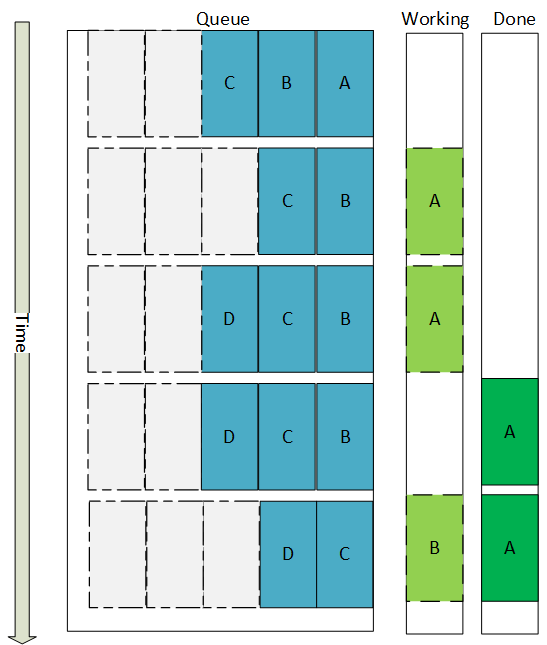
\includegraphics[scale=.75]{img/FIFO_drawing.png}
    \caption{Illustration of FIFO requests are received and processed.}
    \label{fig:fifo_drawing}
\end{figure}
This can be scaled to have multiple workers and distribute the workload, as such the length of the queue will be dependant on the number of requests we can process at a time, the amount of time each request takes to process, and the number of requests in front in the queue.

\subsection{Weighted fair queuing}
Weighted fair queuing (WFQ) is a priority based system, where one specifies a priority based on a set of rules. This is heavily used in networking to implement Quality of Service (QoS) policies, this ensures that even if there are larger jobs sending a bigger flow of traffic, such as a file transfer, low-volume traffic is still transmitted in a timely fashion. \cite{cisco_wfq} Figure \ref{fig:wfq_drawing} show a general overview of what a WFQ can look like; we have requests arriving through one or more pipes, each request is then classified against the rule set and the request is then put in their respective priority queues.
\begin{figure}
    \centering
    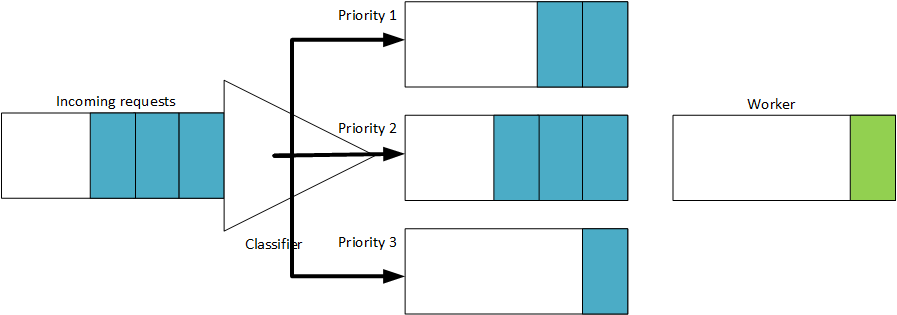
\includegraphics[scale=.5]{img/WFQ_drawing.png}
    \caption{Figure showing an overview of a weighted fair queuing based system with three priority levels}
    \label{fig:wfq_drawing}
\end{figure}
Then based on a cycle we will normally pull from the highest priority, but with time interval $n$ we pull from priority two, and time interval $m | m>n$ we pull from priority three, and so forth for all queues. For example for a telemarketer, you would place Voice over IP (VOIP) as a priority one, file transfers as priority two, all else priority three. This would assure that VOIP would get the most time on the network, while file transfers and other background transmission would still get their fair share at a lower priority.



\pagebreak\section{GPU}
A Graphical Processing Unit (GPU) is specialized hardware designed to accelerate the manipulation of computer graphics and image processing. Compared to a Central Processing Unit (CPU) which is designed and optimized to compute operations in a series. A GPU is massively optimized for parallelism, since for instance calculation of individual pixel colors on screen are entirely independent for each pixel.\cite{gpu_paper} The GPU is built up by multiple simple cores, for instance NVIDIA Kepler GK110/120 contains 192 single-precision CUDA cores and 64 double-precision CUDA cores \cite[p.9]{nvidia_kepler}, each having its own arithmetic logic unit (ALU) and floating point unit (FPU).
\begin{figure}[H]
    \centering
    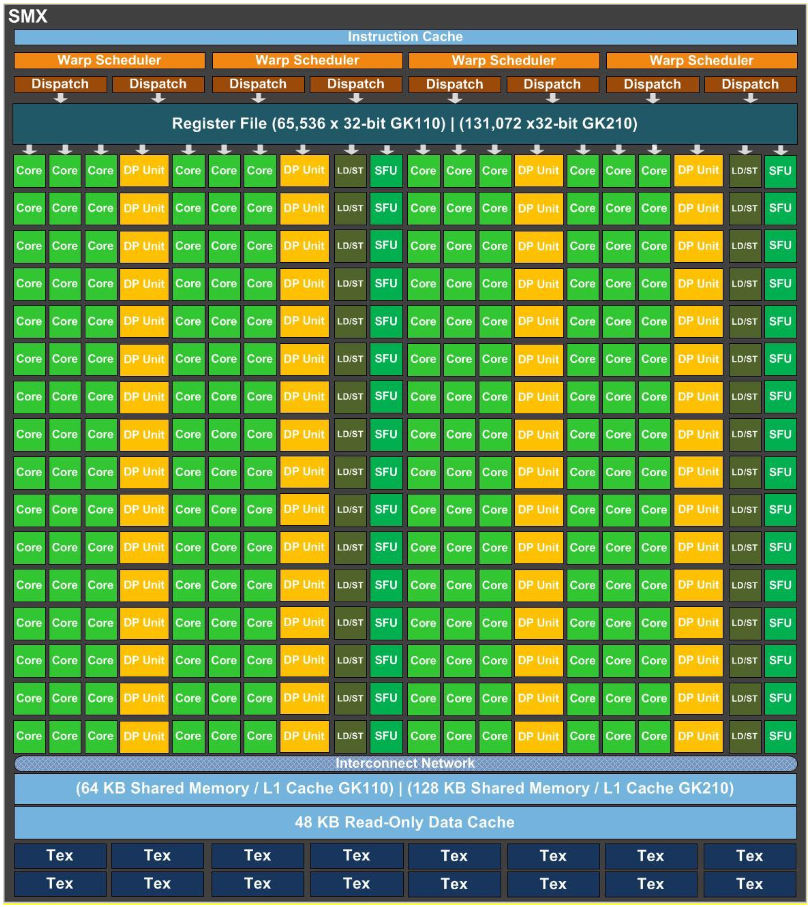
\includegraphics[scale=.6]{img/SMXNvidia.PNG}
    \caption{The architecture of an NVIDIA Kepler GPU. Sourced: NVIDIA \cite{nvidia_kepler}}
    \label{fig:SMXNvidia}
\end{figure}
The GPU shares a major bottleneck with the CPU; limited memory. As with the CPU, each core processes data saved in registries, which are of fairly small size. For instance on Kepler GK110 this is configurable with an initial 64KB on-chip memory that can be split into L1 cache and shared memory.\cite[p13-14]{nvidia_kepler} Including the normal buffers, there is also on-board memory to save on time loading from main memory, or disk.
\begin{figure}
    \centering
    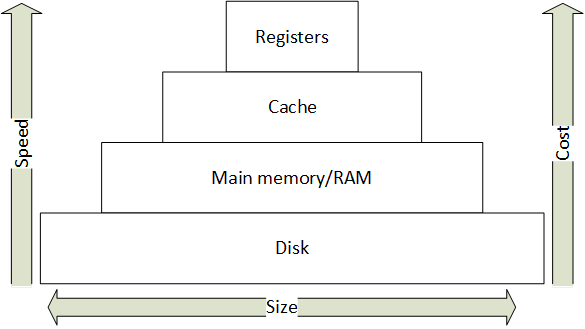
\includegraphics[scale=.7]{img/memory_hierarchy.png}
    \caption{The memory hierarchy showing the different factors of memory with regards to speed, cost, size, and how they influence each other.}
    \label{fig:memory_hierarchy}
\end{figure}
Given the nature of artificial intelligence which is mostly statistics and linear algebra, this leads well into the usage of GPUs to accelerate the learning process. A GPU is specialized in multiprocessing and is great for matrix and vector calculations. It is thus intuitive that increasing the amount of GPU capacity will have a great effect on efficiency: This is shown by Dr. Donald Kinghorn as he measured the efficiency of using distributed GPUs for a Long term-short term memory (LSTM) network where he observed a 5.36 times increase from 1 to 8 GPUs. \cite{puget_tensorflow}
\begin{figure}[H]
    \centering
    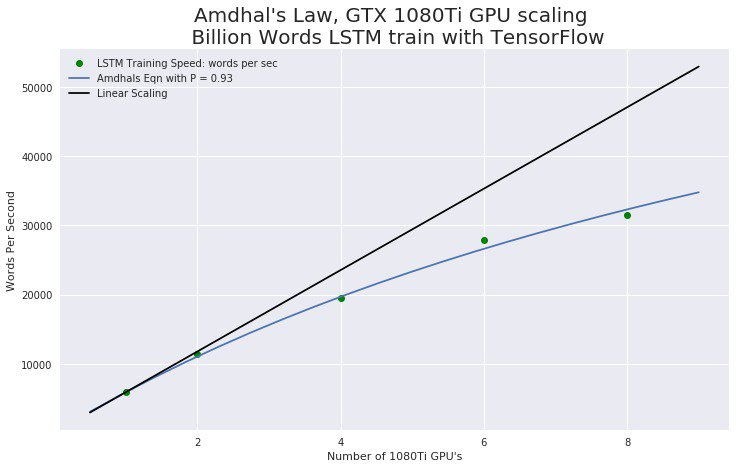
\includegraphics[scale=.5]{img/puget_tensor.jpg}
    \caption{Plot showing the increase in words per second processing as GPU count increases on a LSTM network. Sourced: Donald Kinghorn \cite{puget_tensorflow}}
    \label{fig:puget_tensorflow}
\end{figure}
This follows Amdahl's law with a 93.5\% parallelism, which is defined as 
\[
    S_\text{latency}(s) = \frac{1}{(1-p)+\frac{p}{s}}
\]
where $p$ is the proportion of execution that benefits from parallelism, and $s$ is the number of GPUs. Testing from IBM also shows the increased efficiency on Distributed Deep Learning, running up to 256 GPUs on the ResNet-50 model they saw up to 95\% efficiency increase with 256 GPUs as shown in figure \ref{fig:ibm_tensorflow}. \cite{ibm_tensorflow}
\begin{figure}[H]
    \centering
    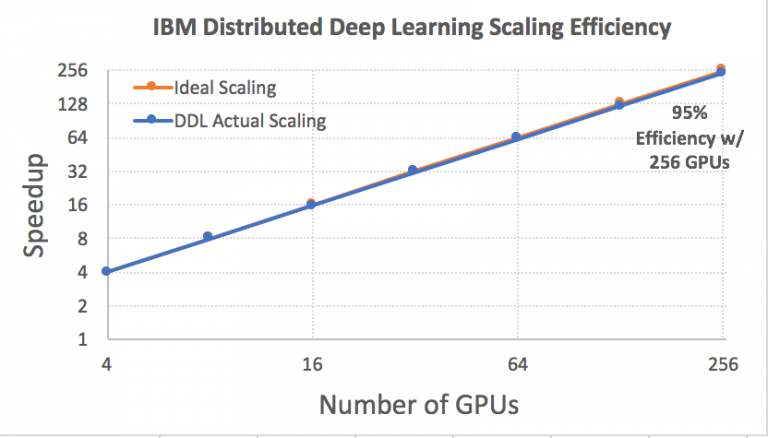
\includegraphics[scale=.5]{img/ibm_resnet.png}
    \caption{Scaling results from IBMs test of ResNet-50 with increasing amount of GPUs. Sourced: IBM \cite{ibm_tensorflow}}
    \label{fig:ibm_tensorflow}
\end{figure}
The sub linear scaling is natural as not all code execution can be ran in parallel, as well as the overhead to distribute the data to the cluster. This is coherent with Amdahl's law as
\[
    \lim_{s\to\infty}S_\text{latency}(s) = \frac{1}{1-p}
\]
shows that as the amount of resources,$s$, increases we are left with the factor of the amount of work that can be done in parallel.


\pagebreak\section{Containerization and Docker}

\subsection{Containerization}

\begin{quote}
"Containerization is a type of virtualization strategy that emerged as an alternative to traditional hypervisor-based virtualization. As with the latter, container-based virtualization involves creating specific virtual pieces of a hardware infrastructure."
\cite{containerization_def}
\end{quote}

\noindent With containerization, a container might feel like a virtual machine, since it has its own networking device and process space so it can create processes like how a virtual machine would. 
However this is not the case, as a container uses the host kernel,which in turn means that means that you can't use different operating system than what the host is running. This is due to how the container is allocating its resources with control groups \cite{cgroup}. 

\subsection{Docker}
Docker is a software that is widely used to make containers, and has in the recent years increased in popularity due to its innovative way of making containers. The way Docker makes it possible to make a container, makes it easier than how it has been before. With Docker you can make what is called a Dockerfile which consist of a set of simple instructions that will be parsed by Docker to be executed in a container to then create a Docker image.

\pagebreak\subsubsection*{Dockerfile}
When creating a container, you will start out with a so called Dockerfile \cite{dockerfile}. The Dockerfile is nothing more than a text file with instructions that Docker recognizes to generate the layers that builds up the image. Figure \ref{fig:Dockerfile} shows how a basic Dockerfile looks like.

\begin{figure}[H]
    \inputminted[linenos]{vim}{code/Dockerfile}
    \caption{An example for a Dockerfile}
    \label{fig:Dockerfile}
\end{figure}

As shown in figure \ref{fig:Dockerfile} one can see that there are four types of instructions\cite{dockerfile} in use in this case, exists more than shown.
\begin{itemize}
    \item \mintinline{vim}|FROM| - Determines what base image you will start from, you can choose to start from a minimalistic image with few packages or bigger images with more packages to minimize the amount of lines in your Dockerfile.
    \item \mintinline{vim}|RUN| - Run executes commands like getting packages from an external repository through for example \mintinline{bash}|apt|
    \item \mintinline{vim}|CMD| - This instruction provides a default command to execute when the container has started.
    \item \mintinline{vim}|EXPOSE| - Tells the Docker what port the container needs to expose and thus listen on
\end{itemize}


\subsubsection*{Docker Image}
A Docker image\cite{dockerimage} consists of multiple small layers that in the end compiles into what is the Docker image. When making a Docker Image you will have something like a Dockerfile as shown in the figure \ref{fig:Dockerfile}, for each line you add to the file it will be added as a new layer to the Docker container and is often called a container layer as it is a thin layer on top which is writable by the container.% fylle dette litt mer ut ang laget på toppen

% KKOOL 
\subsubsection*{Docker Compose}
\begin{quote}
"Compose is a tool for defining and running multi-container Docker applications" \cite{dockercomp}
\end{quote}

When you need more than one container, for example an application that has dependencies on other services, then you could use a Docker compose file. This would allow that a container can depend on one or multiple services, for example you have an application that need to start a database before it starts the application itself, one would use the variable \mintinline{vim}|depend_on| to wait for the database before starting the application.
However when multiple services are in need of communication with each other, you can reference to a container with its name rather than its IP address, as the IP is by default not static. \cite{composeNett}

\begin{figure}[H]
    \inputminted[linenos]{octave}{code/docker-compose.yml}
    \caption{An example for a docker-compose.yml}
    \label{fig:docker-compose}
\end{figure}


As shown on the figure \ref{fig:docker-compose} you will see an example of a docker-compose.yml. 


\pagebreak\section{Kubernetes}
Kubernetes, also known as K8s, is an open source system for automating deployment, scaling, and maintenance of container applications, originally developed by Google and released to the public in 2014. \cite{kubernetes_whatis} Kubernetes can be run as a single instance or part of a cluster of multiple servers, and uses a central tool, kubectl, to manage the infrastructure. Figure \ref{fig:kubernetes_overview} shows a brief overview of how a general Kubernetes infrastructure can look like, using a centralized database to store information on the infrastructure and communicating this to the compute nodes through a central API. Kubernetes supports other container environment than Docker, such as rkt and frakti. \cite{kubernetes_cri}

\begin{figure}[H]
    \centering
    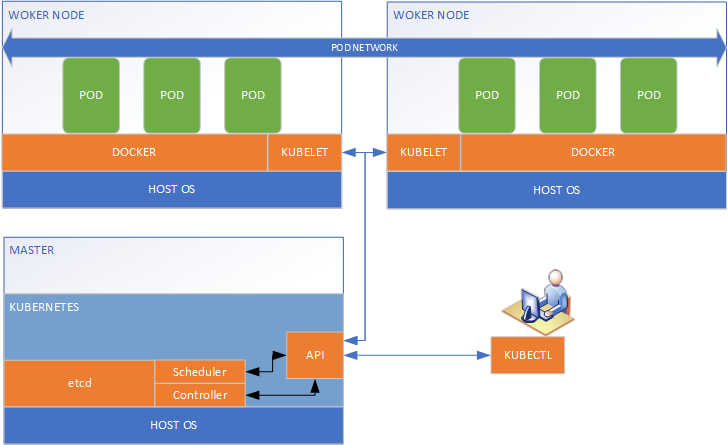
\includegraphics[scale=.75]{img/Kubernetes_overview.png}
    \caption{A brief overview of the Kubernetes infrastructure showing some concepts and parts}
    \label{fig:kubernetes_overview}
\end{figure}

\subsection{Primitives}
\subsubsection*{Node}
A node is a physical- or virtual machine that is part of the Kubernetes cluster which can be scheduled for running one or more pods. Each node needs to have Docker and the kubelet services running. The nodes kubelet service communicates with the master through the API service. \cite{kubernetes_nodes}

\subsubsection*{Pod}
A pod is a group of one or more containers that share storage and networking, and has information on how to run the containers. All containers in the same pod are scheduled at the same time, and to the same node. As such they share namespace and port space, and can access each other through "localhost". \cite{kubernetes_pods} A pod is not intended to be a durable entity, meaning it won't survive node failures, as such a pod is usually deployed through a deployment and not a single entity. One can also specify DNS policies on each pod
\begin{itemize}
    \item \textbf{Default}\\
            The pod inherits the name resolution from the node it is running on. It is important to note that the default is not actually the default if none is specified - this is the ClusterFirst.
    \item\textbf{ClusterFirst}\\
            If the DNS query is within the cluster namespace it will use the clusters DNS service first, else it will forward to the upstream nameserver inherited from the node it is running on.
    \item\textbf{None}\\
            Allows the pod to ignore the DNS settings from the Kubernetes environment, and one is supposed to specify the DNS settings to be used through a custom \mintinline{vim}|dnsConfig|
\end{itemize}

\subsubsection*{Deployment}
A deployment specifies a desired state for a set of resources such as pods, meaning we can use a deployment to specify a set number of pods to run under said deployment. As such if a node fails with a pod from the deployment, it will create a new pod to keep the requirement. \cite{kubernetes_deployments} We can also specify having more than one replica of a pod, if you want to load balance an application adjusting the number of replicas will handle this.

\subsubsection*{Service}
A service is an abstraction that defines a set of pods and a policy as to how to access them. Since pods can die, be born and not be recreated their internal IP addresses will change. A service will then dynamically based on labels ensure that there is a central point to which one can access the pods. \cite{kubernetes_services} For example a deployment containing a front end for an application, one would then create an overlaying service which would give a central ingress point to access the deployments containers.\\\\
Another example is through a concept called \textit{Nodeports}. This maps a port on all hosts in cluster to a specific service which routes traffic to the appropriate pods.


\subsection{Architecture}
\subsubsection*{etcd}
Kubernetes stores the persistent master state in its etcd registry, while all other components watch etcd for changes to bring themselves towards the desired state. Etcd is a distributed key-value store originally developed for CoreOS, but is available open source under the Apache-2.0 license. \cite{openshift_infrastructure, github_etcd}

\subsubsection*{API}
The API is the central communication point for all services that queries the etcd registry. It validates the requests and synchronizes information with the service configurations. \cite{openshift_infrastructure}

\subsubsection*{Scheduler}
The scheduler decides which nodes an unscheduled pod should run on based on resource requirements and available capacity on each node. The node selection can be manipulated through the use of labeling and selectors, user requirements, data locality, and more. \cite{kubernetes_component_overview}

\subsubsection*{Controller manager}
The controller manager is made up by multiple controllers that are run as independent processes on the master system. These include \cite{kubernetes_component_overview}
\begin{itemize}
    \item \textbf{Node Controller}\\
            Responsible for checking and responding when a node goes down
    \item\textbf{Replication Controller}\\
            Maintains the correct number of pods for the deployments that has replication specifications
    \item\textbf{Endpoints Controller}\\
            Handles the "Endpoint objects", meaning it controls the connection between services and pods
    \item\textbf{Service Account \& Token Controller}\\
            Creates service accounts, and controls the access tokens for namespaces.
\end{itemize}

\subsubsection*{Kubelet}
The kubelet is an agent that runs on each node in the cluster. It is responsible for the pods that are allocated to the node are running and healthy based on the pod specification. It does not manage containers that are not created through Kubernetes. \cite{kubernetes_component_overview}

\subsubsection*{kubectl}
Kubectl is a command line interface that provides commands to interact with the Kubernetes cluster and is the main tool when working with Kubernetes. It uses the following syntax 
\mint{vim}|kubectl [command] [TYPE] [NAME] [flags]|
where \mintinline{vim}|command, TYPE, NAME, flags| refer to 
\begin{itemize}
    \item\textbf{command}\\
            Specifies the type of operation to perform on one or more resources, such as\\ \mintinline{vim}|create, get, describe, delete|
    \item\textbf{TYPE}\\
            Specifies the type of resource perform the operation on, such as \mintinline{vim}|pods, deployment, service|
    \item\textbf{NAME}\\
            The name of the resource to perform the operation on, the names are case-sensitive. If the name is not specified, such as \mintinline{vim}|kubectl get pods|, details for all resources are displayed
    \item\textbf{flags}\\
            Specifies optional flags, such as \mintinline{vim}|-o=yaml| to get the output formatted as a YAML object
\end{itemize}
Kubectl contains numerous operations to facilitate the administration of the Kubernetes cluster from just the command line, ranging from pod creation and deletion, to administering service accounts and roles. \cite{kubernetes_kubectl}

\subsubsection*{DNS}
The Kubernetes DNS, or kube-dns, creates a DNS pod and service on the cluster, and makes the kubelets tell individual containers to use the DNS service IP to resolve DNS names. The DNS namespace is only visible inside the cluster unless the DNS service is being specified otherwise. \cite{kubernetes_dns}

\subsubsection*{Cluster networking}
There are third party pod networks that acts as a layer 3 network fabric, an example of this is Flannel from CoreOS. \cite{coreos_flannel}  It runs a simple service called flanneld on each node, and it allocates subnet leases to each host out of a large preconfigured address space.

%\begin{figure}
%    \centering
%    \inputminted[linenos]{yaml}{code/kubernetes_example%.yaml}
%    \caption{an example of a simple kubernetes yaml %file that will create a pod that requires one gpu. %sourced: kubernetes \cite{kubernetes_gpu}}
%    \label{fig:kubernetes_example}
%\end{figure}


\pagebreak\section{Authentication and authorization}
\subsection*{Authentication}
Authentication is the process of confirming someones identity that is using some method to verify that someone is who they say they are by some sort of evidence. In the physical world that could be using your drivers licence to authenticate your identity for example to the police. CompTIA lists authentication methods based on one or more of the following five factors \cite[p. 131]{comptia_sec}
\begin{itemize}
    \item Something you know, such as a password or a PIN number
    \item Something you have, such as a smart card
    \item Something you are, such as fingerprints
    \item Something you do, an action you must do to complete authentication
    \item Somewhere you are, geolocation
\end{itemize}
The most common authentication method is single-factor authentication (SFA), where just one of the methods listed are being used and is most often implemented using a username and password method, where the username is the identity, and the password is something you know.\\
Multi-factor authentication is where you use two or more of the methods above. Note that having two password prompts is not multi-factor. As such a common implementation is using something you know and something you have, in other words a password and a smart card.
\subsection*{Authorization}
Authorization is the process of specifying which access rights an authenticated person has to resources. For example an employee from the economics department should have access to economic data for the company to fulfill his or her job, while an employee working the front desk should not or at the very least have restricted access to only portions involving said employees position. Thus we have the principle of least privilege, this means giving any given user the minimum access such that the user can still fulfill his or her job. \cite[p. 153]{comptia_sec} There is also the principle of separation of duties, meaning that if your job sometimes requires higher privileges than you normally would have, for example a system administrator, you should have different accounts for your normal and administrative work.

\subsection{Methods of authentication}
\subsubsection*{Basic Authentication}
The simplest authentication is the HTTP basic authentication, where the username and password is sent base64 encoded as part of the header using the "Authorization" field. Meaning that one should employ HTTPS over TLS as a means to ensure that the field cannot be read or altered by third parties.
\subsubsection*{OAuth2}
The OAuth2 protocol grants applications or users access to a HTTP service given that they have a valid access token, and that said token is authorized to interact with the requested service. There are two different tokens
\begin{itemize}
    \item \textbf{Access token}\\
            The access token is sent with each request and is used to identify the request owner, and as such validate the authorization given specified by the access control.
    \item \textbf{Refresh token}\\
            The refresh token is issued with the access token, but is only used to renew the access token when it has expired.
\end{itemize}
There are two primary ways to send the access token, either as part of the URL which is not advised as it can then be read in the access logs of the web server, or using the Authorization field in the HTTP header. Compared to the basic authentication standard, OAuth requires the usage of TLS, and recommends at least TLSv1.2 in the specification. \cite{oauth_rfc}
\subsubsection*{Lightweight Directory Access Protocol}
Lightweight Directory Access Protocol (LDAP) is a protocol to contact directory services, such as Microsofts Active Directory or OpenLDAP, over IP. This allows having a centralized system to provide authentication through usernames and passwords which can be used to authenticate to infrastructure or services on the network. LDAP is built up by entries that contain three primary components
\begin{itemize}
    \item\textbf{Distinguished name}\\
            A distinguished name is a unique identifier for the entry and its position in the directory structure
    \item\textbf{Attributes}\\
            Holds metadata about the entry, for instance for a user entry it could be phone number, address, email address.
    \item\textbf{Object classes}\\
            An object class is an element that is used to relate to other objects, such as a group for employees.
\end{itemize}


\pagebreak\section{Microservices}
Microservices is a development technique that focuses on a service-oriented architecture (SOA) such that the application as a whole is a collection of smaller services. Focusing on splitting the application into smaller services makes the application easier to understand, develop and test, and makes modularity easier. It also allows the application to scale the necessary parts of the application, without scaling the whole application. For example a service with an image processing feature that tries to identify objects in an image is slowing down since the instances of image processing is under heavy load and can not keep up. If the image processing is then a singular module, then we can deploy more of these modules without having to scale the rest of the application to handle the increased workload, this under the assumption that additional hardware to support this scaling is available. The important bit is to see that we can scale a single module inside the application, without having to deploy more instances of the whole application, thus giving us more granular control of load balancing the application and as such prioritize where to spend the finite compute power. One can also draw reference to the Unix philosophy as documented by Doug Mcllroy in the 1978 edition of Bell System Technical Journal. Here he laid out the following here retold in short for the full see \cite[p. 8]{bell_unixphilosophy}
\begin{enumerate}
    \item Make each program do one thing well
    \item Expect the output of every program to become the input to another. Do not clutter output, and do not insist on interactive input
    \item Design and build software to be tried early, do not hesitate to throw away clumsy parts and rebuild them
    \item Use tools in preference to unskilled help to lighten a programming task
\end{enumerate}
In short we can see the philosophy is to create small specialized tools that can be coupled together to create a workable application.\\\\

Microservices does have its drawbacks, as denoted by Arnon Rotem-Gal-Oz, he coined the phrase "Nanoservices". \cite{nanoservices} Here he argues that there is a limit as to how fine grained you should make the application, as there is an overhead on inter-process communication as well as from a maintenance perspective. At one point this overhead will outweigh the utility of the service. One of the examples he uses is fragmentation of logic. As applications are broken down into nanoservices the logic flow as you have to traverse multiple services to perform a simple task can become daunting.

\end{document}